\documentclass[11pt]{llncs}

\usepackage{amsmath,amsfonts,amssymb}

\usepackage{microtype}
\usepackage{url}
\usepackage{multirow,subfigure}

\usepackage{xcolor}
\usepackage{tikz}
\usetikzlibrary{arrows}

\usepackage{xspace}
\newcommand{\etal}{\textsl{et al.}\xspace}
\newcommand{\ie}{\textsl{i.e.}\xspace}
\newcommand{\eg}{\textsl{e.g.}\xspace}

\renewcommand\leq\leqslant
\renewcommand\geq\geqslant
\newcommand{\Ot}[1]{{\cal \tilde O}(#1)}

\newcommand{\abs}[1]{\left|#1\right|}
\newcommand{\Z}{{\mathbb Z}}
\newcommand{\R}{{\mathbb R}}

\newcommand{\ceil}[1]{\left\lceil #1 \right\rceil}
\newcommand{\near}[1]{\left\lfloor #1 \right\rceil}
\newcommand{\floor}[1]{\left\lfloor #1 \right\rfloor}

\DeclareMathOperator{\KeyGen}{\ensuremath{\mathsf{KeyGen}}}
\DeclareMathOperator{\Expand}{\ensuremath{\mathsf{Expand}}}
\DeclareMathOperator{\Encrypt}{\ensuremath{\mathsf{Encrypt}}}
\DeclareMathOperator{\Decrypt}{\ensuremath{\mathsf{Decrypt}}}
\DeclareMathOperator{\Recrypt}{\ensuremath{\mathsf{Recrypt}}}
\DeclareMathOperator{\Evaluate}{\ensuremath{\mathsf{Evaluate}}}
\DeclareMathOperator{\Add}{\ensuremath{\mathsf{Add}}}
\DeclareMathOperator{\Mult}{\ensuremath{\mathsf{Mult}}}
\DeclareMathOperator{\Permute}{\ensuremath{\mathsf{Permute}}}
\DeclareMathOperator{\Select}{\ensuremath{\mathsf{Select}}}

\newcommand*\Choose{\ensuremath{\mathsf{Choose}\ }}
\newcommand*\Output{\ensuremath{\mathsf{Output}\ }}
\newcommand*{\poly}{\ensuremath{\mathsf{poly}}}
\newcommand*{\crt}{\ensuremath{\mathsf{CRT}}}

\newcommand*{\pk}{\ensuremath{\mathsf{pk}}}
\newcommand*{\sk}{\ensuremath{\mathsf{sk}}}
\newcommand*{\DGHV}{\ensuremath{\mathsf{DGHV}}}
\newcommand*{\BDGHV}{\ensuremath{\mathsf{BDGHV}}}
\newcommand*{\CDGHV}{\ensuremath{\mathsf{IDGHV}}}
\newcommand*{\FHE}{\ensuremath{\mathsf{FHE}}}

\newcommand*\AddRoundKey{\ensuremath{\mathsf{AddRoundKey}}}
\newcommand*\ShiftRows{\ensuremath{\mathsf{ShiftRows}}}
\newcommand*\SubBytes{\ensuremath{\mathsf{SubBytes}}}
\newcommand*\MixColumns{\ensuremath{\mathsf{MixColumns}}}
\newcommand*\GF{\ensuremath{\mathrm{GF}}}

\newcommand*\D{\ensuremath{\mathcal D}}
\renewcommand*\O{\ensuremath{\mathcal O}}
\newcommand{\keywords}[1]{\par\addvspace\baselineskip
  \noindent\keywordname\enspace\ignorespaces#1.}

\DeclareMathOperator{\im}{\ensuremath{\text{im}}}
  
\newcommand*\bwbs{byte-wise bitslicing\xspace}
\newcommand*\swbs{state-wise bitslicing\xspace}

\newcommand\ignore[1]{}
  
\title{Batch Fully Homomorphic Encryption over the Integers\thanks{This paper is a merger of two independent works~\cite{CLT2013a,KLYC2013} built on the same basic idea but with different contributions. The respective full versions are posted on ePrint.}}

\author{
 Jung Hee Cheon\inst{1}
 \and Jean-S\'ebastien Coron\inst{2}
 \and Jinsu Kim\inst{1}
 \and Moon Sung Lee\inst{1}
 \and Tancr\`ede Lepoint\inst{3,4}
 \and Mehdi Tibouchi\inst{5}
 \and Aaram Yun\inst{6}
 }

\institute{
  Seoul National University (SNU), Republic of Korea\\
  \email{\{jhcheon,kjs2002,moolee\}@snu.ac.kr}\and
  Tranef, France\\
  \email{jscoron@tranef.com}
  \and CryptoExperts, France
  \and \'Ecole Normale Sup\'erieure, France\\
  \email{tancrede.lepoint@cryptoexperts.com}
  \and NTT Secure Platform Laboratories, Japan\\
  \email{tibouchi.mehdi@lab.ntt.co.jp}
  \and Ulsan National Institute of Science and Technology (UNIST), Republic of Korea\\
  \email{aaramyun@unist.ac.kr}
}

\spnewtheorem{cl}{Claim}{\bfseries}{\itshape}

\begin{document}
\maketitle

\begin{abstract}
We extend the fully homomorphic encryption scheme over the integers of van
Dijk~\etal (DGHV) to batch fully homomorphic encryption,
\ie~to a scheme that supports encrypting and homomorphically processing a
vector of plaintexts as a single ciphertext.

We present two variants whose semantic security is based on different
assumptions. One variants removes the additional noise of the DGHV scheme and
introduces a new decisional problem, the Decisional Ap\-pro\-xi\-ma\-te-GCD problem,
whereas the other variant is based on the computational Error-Free
Approximate-GCD but requires a linear sum with additional public key elements.

We also show how to perform arbitrary permutations on the underlying plaintext
vector given the ciphertext and the public key. Our scheme offers competitive
performance: we describe an implementation of the fully homomorphic evaluation
of AES encryption, with an amortized cost of about 12 minutes per AES
ciphertext on a standard desktop computer; this is comparable to the timings
presented by Gentry~\etal at Crypto 2012 for their implementation of a 
Ring-LWE based fully homomorphic encryption scheme.

\keywords{Fully Homomorphic Encryption, Batch Encryption, Homomorphic AES}
\end{abstract}


%%%%%%%%%%%%%%%%%%%%%%%%%%%%%%%%%%%%%%%%%%%%%%%%%%%%%%%%%%%%%%%%%%%%%%%%%%%%%%%%%%%%%%%%%%%%
\section{Introduction}
\label{sec:intro}
%%%%%%%%%%%%%%%%%%%%%%%%%%%%%%%%%%%%%%%%%%%%%%%%%%%%%%%%%%%%%%%%%%%%%%%%%%%%%%%%%%%%%%%%%%%%

\subsubsection{Fully Homomorphic Encryption (FHE).}

Fully homomorphic encryption allows a worker to perform implicit
additions and multiplications on plaintext values while exclusively
manipulating encrypted data. The first construction of a fully
homomorphic scheme (based on ideal lattices) was described by Gentry
in~\cite{GenPhD}, and proceeds in several steps. First, one constructs a
\emph{somewhat homomorphic} encryption scheme, which only supports a limited
number of multiplications: ciphertexts contain some noise that becomes
larger with successive homomorphic multiplications, and only ciphertexts
whose noise size remains below a certain threshold can be decrypted
correctly. The second step is to \emph{squash} the decryption procedure
associated with an arbitrary ciphertext so that it can be expressed as a
low degree polynomial in the secret key bits. Then, Gentry's key
idea, called \emph{bootstrapping}, consists in homomorphically evaluating
this decryption polynomial on encryptions of the secret key bits,
resulting in a different ciphertext associated with the same plaintext,
but with possibly reduced noise. This \emph{refreshed} ciphertext can then
be used in subsequent homomorphic operations. By repeatedly refreshing
ciphertexts, the number of homomorphic operations becomes unlimited,
resulting in a fully homomorphic encryption scheme.

Since Gentry's breakthrough result, many improvements have been made,
introducing new variants, improving efficiency, and providing new
features. Recently, Brakerski, Gentry and Vaikuntanathan described a
different framework where the ciphertext noise grows only linearly with
the multiplicative level instead of exponentially~\cite{BGV2012}, so that
bootstrapping is no longer necessary to obtain a scheme supporting the
homomorphic evaluation of any given polynomial size circuit. Currently
three main families of fully homomorphic encryption schemes are known:

\begin{enumerate}
\item Gentry's original scheme~\cite{GenPhD} based on ideal
  lattices.  An implementation of Gentry's scheme was proposed by
  Gentry and Halevi
  in~\cite{GH2011} with a public key of $2.3$ GB and a ciphertext
  refresh procedure of $30$ minutes; the implementation is based on
  many interesting algorithmic
  optimizations, including some borrowed from Smart and Vercauteren~\cite{SV2010}.

\smallskip

\item van Dijk, Gentry, Halevi and Vaikuntanathan's (DGHV) scheme over the
  integers~\cite{vDGHV2010}. It was recently shown how to significantly
  reduce the public key size in DGHV, yielding a $10.3$ MB public key and
  an $11$-minute refresh procedure~\cite{CNT2012}.

\smallskip

\item Brakerski and Vaikuntanathan's scheme based on the Learning with
  Errors (LWE) and Ring Learning with Errors (RLWE)
  problems~\cite{BV2011a,BV2011b}, and follow-up works (\eg the scale-free variant of Brakerski~\cite{Bra2012} and the NTRU-variant~\cite{LTV2012}). An implementation is described in~\cite{GHS2012c} with an 
  efficient (given the current state of knowledge)
  homomorphic evaluation of the full AES encryption circuit.  The
  authors use the \emph{batch} RLWE-based scheme proposed in~\cite{BGV2012,GHS2012a},
  that allows one to
 encrypt vectors of plaintexts in a single ciphertext and to
 perform any permutation on the underlying plaintext vector while
 manipulating only the ciphertext~\cite{SV2011}. 
\end{enumerate}

\subsubsection{Our Contributions.} 

In this paper we focus on the DGHV scheme. Our goal is to extend DGHV to
support the same batching capability~\cite{SV2011} as in RLWE-based
schemes~\cite{BV2011a,BV2011b}, and to homomorphically evaluate a full AES
circuit with roughly the same level of efficiency as~\cite{GHS2012c}, in
order to obtain an implementation of a FHE scheme with similar features
but based on different techniques and assumptions. 

In the original DGHV scheme, a ciphertext has the form
$$ c= q \cdot p + 2r+m$$
where $p$ is the secret key, $q$ is a large random integer, and $r$ is
a small random integer (noise); the bit message $m\in\{0,1\}$ is recovered by computing
$m=[c \bmod p]_2$.  The scheme is clearly homomorphic for both addition
and multiplication, since addition and multiplication of ciphertexts
correspond to addition and multiplication of plaintexts modulo
$2$. 

To encrypt multiple bits $m_i$ into a single
ciphertext $c$, we use the Chinese Remainder
Theorem with respect to a tuple of $(\ell+1)$ coprime integers $q_0,p_0,\ldots,p_{\ell-1}$. The batch ciphertext has the form
\[ c = \crt_{q_0,p_0,\ldots,p_{\ell-1}}(q, 2r_0+m_0,\ldots,2r_{\ell-1}+m_{\ell-1}), \]
and correctly decrypts to the bit vector $(m_i)$ given by $m_i=[c \bmod p_i]_2$ for all $0 \leq i < \ell$.\footnote{We denote by 
$\crt_{q_0,p_0,\ldots,p_{\ell-1}}(q,a_0,\ldots,a_{\ell-1})$ the unique
  integer $u$ smaller than $q_0\cdot\prod_{i=0}^{\ell-1} p_i$ such that $u\bmod q_0=q$ and $u\bmod p_i=a_i$ for
  all $0 \leq i < \ell$.} Modulo each of the $p_i$'s the
ciphertext $c$ behaves as in the original DGHV scheme. Accordingly, the
addition or multiplication of two ciphertexts yields a new ciphertext
that decrypts to the componentwise sum or product mod $2$ of the original
plaintexts.

The main challenge, however, was to prove the semantic security of our new scheme. In the original DGHV scheme, public-key encryption is
performed by masking the message $m$ with a random subset sum of the
public key elements $x_j=q_j \cdot p + r_j$ as
\begin{equation}
\label{eq:c}
c = \bigg[ m+2r+2 \sum\limits_{j \in S} x_j \bigg]_{x_0}\;.
\end{equation}
The semantic security is proved by applying the Leftover Hash Lemma on
the subset sum, and using the random $2r$ in \eqref{eq:c} to further
randomize the ciphertext modulo $p$.

In Section~\ref{sec:batch-decisional} we explain how we can circumvent this
additional noise $2r$ in the classical DGHV scheme by relying on a new
decisional problem, the Decisional Approximate-GCD. Extending DGHV public-key
encryption to the batch setting may at first seem straightforward: one can use
a similar random subset sum technique in the batch variant by generating
public key elements $x_j$ with a small residue modulo each of the $p_i$'s
instead of only modulo $p$. The generalization of the proof to the batch
scheme is then straightforward. We show that our batch DGHV scheme
can encrypt $\ell=\Ot{\lambda^2}$ bits in a single ciphertext; therefore
the ciphertext expansion ratio becomes $\Ot{\lambda^3}$ instead of
$\Ot{\lambda^5}$ in the original scheme.

Unfortunately this approach relies on a \emph{new} decisional problem. In Section~\ref{sec:batch-error-free}, we present a variant of the batch scheme relying on the known Error-Free Approximate-GCD problem, that is a computational problem as in all previous instances of the DGHV schemes~\cite{vDGHV2010,CMNT2011,CNT2012}. For the proof of semantic security to go through, the ciphertext $c$
should be independently randomized modulo each of the $p_i$'s, which isn't easy to achieve without knowing the $p_i$'s. Indeed, if we only use a single additive term $2r$ as in~\eqref{eq:c}, then the \emph{same} random term $2r=2r \bmod p_i$ is added modulo each of the $p_i$, which breaks the security proof. We provide thus a ``correct'' generalization of the semantic security of DGHV to the batch setting relying on a computational problem. This is
done by replacing the term $2r$ in
\eqref{eq:c} by another subset sum of public key elements which, taken
modulo each of the $p_i$'s, generate a lattice with special properties.
Our security proof then applies the Leftover Hash Lemma modulo this
lattice instead of only modulo $q_0$.

In addition to componentwise addition and multiplication, we also show
how to perform any permutation on plaintext bits publicly. As opposed
to~\cite{BGV2012,GHS2012a}, we cannot use an underlying algebraic
structure to perform rotations over plaintext bits (clearly, the
automorphisms of $\Z$ do not provide any useful action on ciphertexts).
Instead we show how to perform arbitrary permutations on the plaintext
vector during the ciphertext refresh operation at no additional cost (but with
a slight increase of the public key size). Notice also that the $\Recrypt$
operation is done in parallel over the 
$\ell$ slots, with the same complexity as a single $\Recrypt$
operation in the original scheme.

Finally, we describe an implementation of our batch DGHV scheme of Section~\ref{sec:batch-error-free}, with
concrete parameters. We use our batch DGHV scheme to homomorphically
evaluate the full AES encryption circuit. For the ``Large'' parameters
with $\geq72$ bits of security, our implementation  homomorphically
encrypts up to  $531$ AES ciphertexts in parallel in an amortized $12$
minutes per AES ciphertext on a desktop computer. This is comparable to
the timings presented by Gentry~\etal at Crypto 2012 for their
implementation of an RLWE-based scheme~\cite{GHS2012c}.\footnote{
Notice that our implementation uses bootstrapping whereas the implementation
of~\cite{GHS2012c} just used a somewhat homomorphic encryption scheme which
could cope with a huge depth. }

While our batch variant of DGHV does not provide additional features nor
significantly improved efficiency over the RLWE-based scheme of~\cite{GHS2012a}, we believe it is interesting to obtain FHE schemes with
similar properties but based on different techniques and assumptions.  


%%%%%%%%%%%%%%%%%%%%%%%%%%%%%%%%%%%%%%%%%%%%%%%%%%%%%%%%%%%%%%%%%%%%%%%%%%%%%%%%%%%%%%%%%%%%
\section{The Somewhat Homomorphic DGHV Scheme}
\label{sec:dghv}
%%%%%%%%%%%%%%%%%%%%%%%%%%%%%%%%%%%%%%%%%%%%%%%%%%%%%%%%%%%%%%%%%%%%%%%%%%%%%%%%%%%%%%%%%%%%

In this section, we recall the somewhat homomorphic encryption scheme
over the integers of van Dijk, Gentry, Halevi and
Vaikuntanathan (DGHV) in~\cite{vDGHV2010}. Let $\lambda$ be the
security parameter, $\tau$ be the number of elements in the public
key, $\gamma$ their bit-length, $\eta$
the bit-length of the secret key $p$ and $\rho$ (resp.\ $\rho'$) the
bit-length of the noise in the public key (resp.\ in a fresh
ciphertext). 

For a real number
$x$, we denote by $\lceil x \rceil$, $\lfloor x \rfloor$ and $\lceil x
\rfloor$ the upper, lower or nearest integer part of $x$. For
integers $z$, $p$ we denote the reduction of $z$ modulo $p$ by
$(z\bmod p)$ or $[z]_p$ with $-p/2 < [z]_p \leq p/2$. 

For a specific $\eta$-bit odd integer $p$, we use the following distribution over $\gamma$-bit integers:
\[ \mathcal{D}_{\gamma,\rho}(p) = \left\{ \begin{array}{c}\Choose q \leftarrow \mathbb{Z} \cap [0,2^\gamma/p),~
r \leftarrow \mathbb{Z} \cap (-2^\rho,2^\rho) :\\ \Output x =
q \cdot p + r \end{array}\right\}. \]

\begin{description}
\item[$\DGHV.\KeyGen(1^\lambda)$.] Generate an $\eta$-bit random prime integer $p$. For $0 \leq i \leq \tau$, sample $
x_i \leftarrow \mathcal{D}_{\gamma,\rho}(p) $. Relabel the $x_i$'s  so
that $x_0$ is the largest. Restart unless $x_0$ is odd and $[x_0]_p$
is even. Let $\pk=(x_0,x_1,\ldots x_\tau)$ and $\sk=p$.
\\\vspace{-0.25cm}
\item[$\DGHV.\Encrypt(\pk, m \in \{0,1\})$.] Choose a random subset $S \subseteq
\{1,2,\ldots,\tau\}$ and a random integer $r$ in
$(-2^{\rho'}, 2^{\rho'})$, and output the ciphertext:
\begin{equation}
\label{eq:DGHV}
 c = \bigg[ m+2r+2 \sum\limits_{i \in S} x_i \bigg]_{x_0}.
\end{equation}
\vspace{-0.25cm}
\item[$\DGHV.\Evaluate(\pk, C, c_1, \ldots, c_t)$.] Given the circuit
$C$ with $t$ input bits and $t$ ciphertexts $c_i$, apply the addition
and multiplication gates of $C$ to the ciphertexts, performing all the
additions and multiplications over the integers, and return the
resulting integer.
\\\vspace{-0.25cm}
\item[$\DGHV.\Decrypt(\sk, c)$.] Output $m \leftarrow [c \bmod p]_2$.
\end{description}

As shown in~\cite{vDGHV2010} the scheme is somewhat homomorphic, \ie a
limited number of homomorphic operations can be performed on
ciphertexts. More precisely given two ciphertexts $c=q \cdot p+2r+m$
and $c'=q' \cdot p+2r'+m'$ where $r$ and $r'$ are $\rho'$-bit
integers, the ciphertext $c+c'$ is an encryption of
$m + m' \bmod 2$ under a $(\rho'+1)$-bit noise and the ciphertext $c \cdot
c'$ is an encryption of $m \cdot m'$ with noise bit-length $\simeq
2 \rho'$. Since the ciphertext noise must remain smaller than $p$ to maintain correctness, 
the scheme roughly allows $\eta/\rho'$ successive multiplications on ciphertexts.

The scheme is semantically secure under the Approximate-GCD assumption
(see~\cite{vDGHV2010}):

\begin{definition}[Approximate GCD]
\label{def:approxGCD}
 The 
  $(\rho,\eta,\gamma)$-Approximate-GCD problem consists, given a random $ \eta $-bit odd integer $ p $ and
  given  polynomially many samples from $ \mathcal{D}_{\gamma,\rho}(p) $, in outputting $p$.
\end{definition}

%%%%%%%%%%%%%%%%%%%%%%%%%%%%%%%%%%%%%%%%%%%%%%%%%%%%%%%%%%%%%%%%%%%%%%%%%%%%%%%%%%%%%%%%%%%%
\section{Batch DGHV Scheme Based on a new Decisional Assumption}\label{sec:batch-decisional}
%%%%%%%%%%%%%%%%%%%%%%%%%%%%%%%%%%%%%%%%%%%%%%%%%%%%%%%%%%%%%%%%%%%%%%%%%%%%%%%%%%%%%%%%%%%%

%\begin{itemize}
%  \item DGHV without additional noise + security proof with new decisional problem
%  \item Extension to batch
%
%\end{itemize}

We describe our first extension of the DGHV scheme for the batch setting.  We extend the DGHV scheme
by packing $\ell$ plaintexts $m_0$, \dots, $m_{\ell-1}$ into a single ciphertext, using Chinese Remainder
Theorem.  Moreover, for somewhat homomorphic encryption, this allows us to encrypt not only bits
but elements from rings of form $\Z_Q$.

Therefore, we encrypt $(m_0, \dots, m_{\ell-1})\in\Z_{Q_0}\times\cdots\times\Z_{Q_{\ell-1}}$ into a ciphertext
of following form:
\[
c=\crt_{q_0,p_0,\ldots,p_{\ell-1}}(q, Q_0 r_0+m_0,\ldots,Q_{\ell-1}r_{\ell-1}+m_{\ell-1}),
\]
where $q$ is uniform random in modulo $q_0$ and $r_i$ are small noises.  Decryption can be done by
\[
m_i=[c\bmod{p_i}]_{Q_i}.
\]
Homomorphic addition and multiplication can be done by corresponding arithmetic operations on ciphertexts.

This scheme can be considered as encryption of vectors $(m_0, \dots, m_{\ell-1})$, supporting parallel, componentwise
addition and multiplications.  Or, if we choose $Q_i$ to be mutually prime, then using the isomorphism 
$\Z_{\prod Q_i}\cong\prod\Z_{Q_i}$, we may regard this as somewhat homomorphic encryption supporting arithmetic operations
on $\Z_Q$, with $Q=Q_0\cdots Q_{\ell-1}$.

In order to allow public-key encryption, we provide integers $x'_i$ and $x_j$ in the public key, such that $x'_i\bmod{p_j}=Q_{j}r'_{i,j}+\delta_{i,j}$, and $x_i\bmod{p_j}=Q_{j}r_{i,j}$ for all $i$, $j$.  Then a plaintext vector $\vec{m}=(m_0, \dots, m_{\ell-1})$ is encrypted as follows:
\[
c=\left[\sum_{i=0}^{\ell-1}m_i\cdot x_i'+\sum_{i\in S} x_i\right]_{x_0}.
\]

As explained in the Introduction, the additional, larger noise $2r$ from the DGHV scheme is not used in this version.
This simplifies the construction, with the tradeoff of a new decisional assumption and larger security loss.  
In Section~\ref{sec:batch-error-free}, we present another version which handles this issue differently.

%%%%%%%%%%%%%%%%%%%%%%%%%%%%%%%%%%%%%%%%%%%%%%
\subsection{Description}
%%%%%%%%%%%%%%%%%%%%%%%%%%%%%%%%%%%%%%%%%%%%%%
\begin{description}\label{CDGHV}
\item[$\CDGHV.\KeyGen(1^\lambda,(Q_j)_{0\leq j <\ell})$.] Choose $\eta$-bit distinct primes $p_j$, $0\leq j<\ell$, and denote $\pi$
their product. Let us define the error-free public key element
$x_0=q_0\cdot\pi$, where $q_0 \gets \Z \cap [0,2^{\gamma}/\pi)$
  is a $2^{\lambda^2}$-rough integer.\footnote{An integer $a$ is $b$-rough when it does
    not contain prime factors smaller than $b$. As in~\cite{CMNT2011} one can
    generate $q_0$ as a product of $2^{\lambda^2}$-bit primes.}  
  Make sure that $\gcd(Q_j,x_0)=1$ for $0\leq j<\ell$, and abort otherwise.
  
  Choose the following integers $x_i$ and $x'_i$ with a quotient by $\pi$ uniformly
  and independently distributed in $\Z\cap [0, q_0)$, and with the
    following distribution modulo $p_j$ for $0 \leq j < \ell$:
$$
\begin{array}{lll}
1 \leq i \leq \tau, & \qquad x_i\bmod p_j = Q_j r_{i,j},& \qquad r_{i,j}
\gets\Z\cap(-2^{\rho}, 2^{\rho}) \\[.2cm]

0\leq i\leq \ell-1, & \qquad x'_i\bmod p_j = Q_jr'_{i,j}+\delta_{i,j}, &
\qquad r'_{i,j}\gets\Z\cap(-2^{\rho}, 2^{\rho}) \\[.2cm]

\end{array}
$$

Finally, let $\pk = \left\langle x_0, \left(Q_i\right)_{0\leq i \leq \ell-1},\left(x_i\right)_{1\leq i\leq \tau}, \left(x'_i\right)_{0\leq i\leq \ell-1}\right\rangle$ and $\sk=(p_j)_{0\leq j\leq {\ell-1}}$.
\\\vspace{-0.25cm}
\item[$\CDGHV.\Encrypt(\pk, {\vec{m}})$.] For any $\vec{m}=(m_0,\dots,m_{\ell-1})$ with $m_i\in\Z_{Q_i}$, choose random binary vector $\vec{b}=(b_i)_{1\leq i \leq \tau}\in \{0,1\}^\tau$, output the ciphertext:
\begin{equation}
\label{eq:enccdghv}
c = \left[\sum\limits_{i=0}^{\ell-1} m_i \cdot x'_i + 
	\sum_{i=1}^\tau 
b_i\cdot x_i\right]_{x_0}.
\end{equation}
\item[$\CDGHV.\Decrypt(\sk, c)$.] Output $\vec{m}=(m_0,\ldots,m_{\ell-1})$ where $m_j \gets [c]_{p_j} \bmod Q_j$.
\\\vspace{-0.25cm}
\item[$\CDGHV.\Add(\pk, c_1, c_2)$.] Output $c_1+c_2 \bmod x_0$
\\\vspace{-0.25cm}
\item[$\CDGHV.\Mult(\pk, c_1, c_2)$.] Output $c_1 \cdot c_2 \bmod x_0$.
\end{description}
%%%%%%%%%%%%%%%%%%%%%%%%%%%%%%%%%%%%%%%%%%%%%%
\subsection{Parameters and Correctness}\label{parameter}
%%%%%%%%%%%%%%%%%%%%%%%%%%%%%%%%%%%%%%%%%%%%%%
Roughly speaking, $\ell$ determines the size of the message space.
The binary length of $Q_j$ can be an integer from $2$ to $\eta/8$ depending on the multiplicative depth of the scheme. The details of analysis are given in Appendix~\ref{app:correctness}.
The parameters should satisfy the following constraints: 
\begin{itemize}
\renewcommand{\labelitemi}{\tiny $\bullet$}
\itemsep.4em
\item $\rho=\tilde{\mathcal{O}}(\lambda)$, to be secure against Chen-Nguyen's attack~\cite{CN2012} and Howgrave-Graham's attack~\cite{How2001},
\item $\eta=\tilde{\Omega}(\lambda^2 +\rho\cdot \lambda)$, to resist the factoring attack using the elliptic curve method~\cite{Len1987} and to permit enough multiplicative depth (in Appendix~\ref{app:correctness}),
\item $\gamma=\eta^2\omega(\log \lambda)$, to resist Cohn and Heninger's attack~\cite{CH2011} and the attack using Lagarias algorithm~\cite{Lag1985} on the approximate GCD problem,
\item $\tau=\gamma+\omega(\log\lambda)$, in order to use left-over hash lemma in the security proof which is given in Section~\ref{reduce_acd}.
\end{itemize}
We choose $\gamma=\tilde{\mathcal{O}}(\lambda^5), \eta=\tilde{\mathcal{O}}(\lambda^2),
\rho=2\lambda$, $\tau=\gamma+\lambda$ which is similar to the DGHV's convenient parameter setting \cite{vDGHV2010}. We remark that $b_i$ can be chosen in the much larger interval so as to reduce the public key size as in Section~\ref{sec:batch-error-free}. 

The following lemma is proven in Appendix~\ref{app:correctness} with the definition of correctness for
homomorphic encryption schemes, with respect to a set
$\mathcal{C_E}$ of permitted circuits.

\begin{lemma}\label{lem:correctness}
The above scheme is correct for $\mathcal{C_E}$.
\end{lemma}

%%%%%%%%%%%%%%%%%%%%%%%%%%%%%%%%%%%%%%%%%%%%%%
\subsection{Semantic Security}\label{reduce_acd}
%%%%%%%%%%%%%%%%%%%%%%%%%%%%%%%%%%%%%%%%%%%%%%

Here we show the security of the \CDGHV\ scheme.  In order to prove this, we introduce a new assumption called $\ell$-$\mathbf{DACD}_Q$, and give a security proof based on this assumption.  In fact, this rather complicated assumption is given only as an intermediate step for the proof, and in Section~\ref{decisional_assumption}, we prove this assumption from a simpler decisional assumption.

Given two integer vectors $\vec{p}=(p_0, \dots, p_{\ell-1})$, $\vec{Q}=(Q_0, \dots, Q_{\ell-1})$ of length $\ell$ and an integer $q_0$, let us define the distribution $\D_\rho(\vec{p}; \vec{Q}; q_0)$ as follows.  The output of the distribution is
\[
x=\crt_{q_0,p_1,\dots,p_k}(q,Q_0r_0,\dots,Q_{\ell-1}r_{\ell-1}),
\]
where $q\gets\Z\cap[0,q_0)$ and $r_i\gets\Z\cap(-2^\rho,2^\rho)$ for $i=0,\dots,\ell-1$

\begin{definition}[$\ell$-Decisional Approximate $\mathbf{GCD}_Q$ Problem: $\ell$-$\mathbf{DACD}_Q$] \\
The $(\rho,\eta,\gamma,\mu)$-$\ell$-decisional approximate GCD$_Q$ problem is: for $\eta$-bit distinct primes $p_0,\dots,p_{\ell-1}$ and $\mu$-bit integers $Q_0,\dots,Q_{\ell-1}$, given a $\gamma$-bit integer  $x_0:=q_0p_0\cdots p_{\ell-1}$, with $\gcd(x_0,Q_i)=1$ for $i=0,\dots,\ell-1$, and  %$q_0=\Big\lfloor{2^\gamma\over\prod_{i=1}^kp_i}\Big\rfloor$ , 
polynomially many samples from $\D:=\D_{\rho}(\vec{p};\vec{Q};q_0)$ and a set $X$ consisting of $\ell$ integers $x'_i=\crt_{q_0,p_0,\dots,p_{\ell-1}}(q_i,Q_0r'_{i,0}+\delta_{i,0},\dots,Q_{\ell-1}r'_{i,\ell-1}+\delta_{i,\ell-1})$ where $q_i$, $r'_{i,j}$ are chosen by
$q_i\gets\Z\cap[0,q_0)$, $r'_{i,j}\gets\Z\cap(-2^\rho,2^\rho)$, determine $b\in\{0,1\}$ from $z=x+r\cdot b\mod x_0$ where $x\gets\D$ and $r\gets\Z\cap[0,x_0)$.
\end{definition}

The $(\rho,\eta,\gamma,\mu)$-$\ell$-decisional approximate GCD$_Q$ assumption then states that this problem is hard for any polynomial time distinguisher.

\begin{theorem}
The \CDGHV\ scheme is semantically secure under the $l$-decisional approximate $\mathrm{GCD}_Q$ assumption.
\end{theorem}
\begin{proof}
We provide a sketch of the proof.  See the complete proof in the full version~\cite{KLYC2013}.

Essentially, the idea of the proof is that the \CDGHV\ scheme is a lossy encryption~\cite{BHY2009}.  Both the correctly generated public key $\pk$ and the lossy key $\pk'$ have the following form
\[
\left\langle x_0, \left(Q_i\right)_{0\leq i \leq \ell-1},\left(x_i\right)_{1\leq i\leq \tau}, \left(x'_i\right)_{0\leq i\leq \ell-1}\right\rangle,
\]
but note that, for the real public key $\pk$, $x_i$ are chosen as $x_i\gets\D_\rho(\vec{p}; \vec{Q}; q_0)$,
and for the lossy public key $\pk'$, $x_i\gets\Z\cap[0,x_0)$.

Now we may rely on the standard hybrid argument to show that $\pk$ and $\pk'$ are computationally indistinguishable, under the $(\rho,\eta,\gamma,\mu)$-$\ell$-decisional approximate GCD$_Q$ assumption: for each $\hat\i\in\{1, \dots, \tau\}$, we define $\pk^{(\hat\i)}$, where
\[
x_i \gets \begin{cases}
\Z\cap[0,x_0)&\text{for $i\leq \hat\i$},\\
\D_\rho(\vec{p}; \vec{Q}; q_0)&\text{for $i>\hat\i$}.
\end{cases}
\]
Then $\pk^{(0)}$ is identical as $\pk$, and $\pk^{(\tau)}$ is identical as $\pk'$, and using the $(\rho,\eta,\gamma,\mu)$-$\ell$-decisional approximate GCD$_Q$ assumption, we may show that $\pk^{(\hat\i)}$ is indistinguishable from $\pk^{(\hat\i+1)}$ for $\hat\i=0$, \dots, $\tau-1$,
proving that $\pk$ and $\pk'$ are computationally indistinguishable.

Next, we show that under the lossy key $\pk'$, the \CDGHV\ scheme is secure statistically: for any two plaintexts $\vec{m}$ and $\vec{m}'$, the distributions of their corresponding ciphertexts $c$, $c'$ under the lossy key $\pk'$ are statistically close.  Recall that from equation~\ref{eq:enccdghv}, we have
\begin{equation*}
c = \left[\sum\limits_{i=0}^{\ell-1} m_i \cdot x'_i + 
	\sum_{i=1}^\tau 
b_i\cdot x_i\right]_{x_0}.
\end{equation*}

Now, when we choose $x_i$ from the lossy public key $\pk'$, $x_i$ are uniform on $\Z\cap[0,x_0)$, and we may use the leftover hash lemma.  In fact we may use the simplified version shown in Lemma~1 of~\cite{vDGHV2010} to conclude that the distribution of $[\sum_{i=1}^\tau b_i\cdot x_i]_{x_0}$ is statistically close to the uniform distribution on $\Z\cap[0,x_0)$, when the parameters are chosen according to Section~\ref{parameter}.  Therefore, the distribution of $c$ is uniform random, regardless of the plaintext vector $\vec{m}$.  This shows that \CDGHV\ is a lossy encryption scheme, and the semantic security directly follows from that.\qed
\end{proof}

%%%%%%%%%%%%%%%%%%%%%%%%%%%%%%%%%%%%%%%%%%%%%%
\subsection{Hardness Assumption}\label{decisional_assumption}
%%%%%%%%%%%%%%%%%%%%%%%%%%%%%%%%%%%%%%%%%%%%%%
The semantic security of our scheme is based on a new decisional assumption of approximate GCD problem. 
%In fact, decisional approximate GCD is considered by Coron et al[] for the first time.
 For two specific
integers $p$ and $q_0$, we use the following distribution over
$\gamma$-bit integers:  
\[ \D_\rho(p,q_0) = \left\{ \Choose q\gets [0, q_0),
  r\gets \Z\cap (-2^\rho, 2^\rho) : \Output y=q\cdot p+r
  \right\}. \] 

\begin{definition}[Decisional Approximate GCD Problem: DACD]
\label{def:dagcd}
The $(\rho,\eta,\gamma)$-decisional approximate GCD problem is: For a random $\eta$-bit prime $p$, given a $\gamma$-bit integer  $x_0=q_0\cdot p$ and polynomially many samples from $\D_{\rho}(p,q_0)$,
%and a set $S:=\{x_i \mod x_0 \big|$ for polynomially many samples $x_i\gets \D_{\gamma,\rho}(p)\}$, 
determine $b\in\{0,1\}$ from $z=x+r\cdot b\mod x_0$ where $x\gets\D_{\rho}(p,q_0)$ and $r\gets\Z\cap[0,x_0)$.
\end{definition}

We give a sketch of the proof of the following lemma. For the detailed proof, see the full version \cite{KLYC2013}. 
\begin{lemma}
\label{le:redsec}
The $\ell$-decisional-Approximate-GCD$_Q$ problem is hard if the
decisional-approximate-GCD problem is hard.
\end{lemma}
\begin{proof}[Sketch]


\end{proof}
\begin{corollary}
The generalized DGHV scheme is semantically secure if the
decisional-approximate-GCD assumption holds.
\end{corollary}

%%%%%%%%%%%%%%%%%%%%%%%%%%%%%%%%%%%%%%%%%%%%%%%%%%%%%%%%%%%%%%%%%%%%%%%%%%%%%%%%%%%%%%%%%%%%
\section{Batch DGHV Scheme Based on the Error-Free Approximate-GCD}\label{sec:batch-error-free}
%%%%%%%%%%%%%%%%%%%%%%%%%%%%%%%%%%%%%%%%%%%%%%%%%%%%%%%%%%%%%%%%%%%%%%%%%%%%%%%%%%%%%%%%%%%%

In this section, we present a generalization of the $\CDGHV$ scheme based on 
the \emph{computational} Error-Free Approximate-GCD problem already used 
in~\cite{vDGHV2010,CMNT2011,CNT2012} rather than on the Decisional 
Approximate-GCD problem (Definition~\ref{def:dagcd}). This is made possible 
by adding a new set of elements in the public key but yields a more intricate 
scheme. For sake of simplicity, we assume that $Q_0=\cdots=Q_{\ell-1}=2$ 
throughout the rest of the paper. Notice however that the security proof of 
this Section extends easily to general $Q_i$'s as in Section~\ref{sec:batch-decisional}.

We recall that, as mentioned in the Introduction, one cannot add a
randomization with $2r$ during encryption in the batch scheme (cf.~Equation~\eqref{eq:enccdghv}) as in the DGHV scheme. Indeed, this randomisation does not work because the \emph{same} random term $2r=2r \bmod p_i$ is added
modulo each of the $p_i$, whereas for the security proof to go through
these random terms should be independently distributed modulo each of the
$p_i$'s. Therefore a new technique is required to extend DGHV to
semantically secure batch encryption.

\paragraph{Variant of the DGHV Scheme.} In the following, we start by describing a variant of DGHV still for a
single bit message $m$ only, but which \emph{does} extend naturally to the
batch setting. We first consider the DGHV scheme without the additional
random $2r$, since this term is of no use in the batch setting. A single
message bit $m$ is then encrypted as
\[
    c = \Big[m + 2\sum\limits_{i\in S} x_i\Big]_{x_0}
\]
where $x_i=q_i \cdot p+r_i$. In order to prove semantic security as in
\cite{vDGHV2010}, one should prove that the values $q$ and $r'$ given by
$c=q \cdot p+2r'+m$ are essentially random and independently distributed.
The randomness of $q=2\sum_{i \in S} q_i \bmod q_0$ follows from the
Leftover Hash Lemma (LHL) modulo $q_0$. However we cannot apply the LHL
to $r'=\sum_{i \in S} r_i$ because it is distributed over ${\mathbb Z}$
instead of modulo an integer. Note that in the original scheme the
randomness of $r'$ followed from adding a random $2r$ in \eqref{eq:c},
much larger than the $r_i$'s.

Let us assume that we could somehow reduce the integer variable
$r'=\sum_{i \in S} r_i$ modulo some integer $\varpi$. Then we could apply
the LHL simultaneously modulo $q_0$ and modulo $\varpi$, and the
distributions of $q \bmod q_0$ and $r' \bmod \varpi$ would be
independently random as required. However, during public-key encryption
we certainly do not have access to the variable $r'=\sum_{i \in S} r_i$,
so we cannot \emph{a priori} reduce it modulo an integer $\varpi$ in the
encryption phase.

Our technique is the following: instead of reducing the variable $r'$
modulo $\varpi$, we add a large random multiple of $\varpi$ to $r'$. This
can be done by extending the public key with a new element $\varPi$ such
that $\varPi \bmod p=\varpi$. Encryption would then be performed as
\begin{equation}
\label{eq:DGHVmod}
c = \Big[m + 2b \cdot \varPi+
  2\sum\limits_{i\in S} x_i\Big]_{x_0}
\end{equation}
for some large random integer $b$. Modulo $p$ this gives a new integer
$r''=r' + b \cdot \varpi$; we argue that this enables to proceed as if
$r'$ was actually reduced modulo $\varpi$. Namely, if we generate the
$r_i$'s such that the sum $r'=\sum_{i \in S} r_i$ is not much larger than
$\varpi$, then reducing $r'$ modulo $\varpi$ would just subtract a
small multiple of $\varpi$, which is negligible compared to the large
random multiple $b \cdot \varpi$. Formally  the distribution of $r' + b
\cdot \varpi$ is statistically close to $(r' \bmod \varpi) + b \cdot
\varpi$, which enables us to apply the LHL to $r' \bmod \varpi$ and
eventually obtain a security proof.

\paragraph{Extension to the Batch Scheme.} Now the advantage of \eqref{eq:DGHVmod} is that it can be easily extended
to the batch setting. Instead of using a single random multiple of
$\varPi$, we use a subset sum of $\ell$ such multiples $\varPi_i$, where
$\varPi_i \bmod p_j=\varpi_{i,j}$. The Leftover Hash Lemma is then
applied modulo the lattice generated by the $\varpi_{i,j}$. This shows
that the random noise values modulo the $p_i$'s follow essentially
independent distributions, and eventually leads to a security proof based on the Error-Free Approximate-GCD problem. 

%%%%%%%%%%%%%%%%%%%%%%%%%%%%%%%%%%%%%%%%%%%%%%
\subsection{Description}\label{subsec:description}
%%%%%%%%%%%%%%%%%%%%%%%%%%%%%%%%%%%%%%%%%%%%%%

\begin{description}
\item[$\BDGHV.\KeyGen(1^\lambda)$.] Generate a collection of $\ell$
random $\eta$-bit primes $p_j$, $0\leq j<\ell$, and denote $\pi$
their product. Let us define the error-free public key element
$x_0=q_0\cdot\pi$, where $q_0 \leftarrow \Z \cap [0,2^{\gamma}/\pi)$
  is a $2^{\lambda^2}$-rough integer.
%  \footnote{An integer $a$ is $b$-rough when it does
%    not contain prime factors smaller than $b$. As in~\cite{CMNT2011} one can
%    generate $q_0$ as a product of $2^{\lambda^2}$-bit primes.}  

  Generate the following integers $x_i$, $x'_i$ and $\varPi_i$ with a quotient by $\pi$ uniformly
  and independently distributed in $\Z\cap [0, q_0)$, and with the
    following distribution modulo $p_j$ for $0 \leq j < \ell$:
$$
\begin{array}{lll}
1 \leq i \leq \tau, & \qquad x_i\bmod p_j = 2r_{i,j},& \\[.2cm]

0\leq i\leq \ell-1, & \qquad x'_i\bmod p_j = 2r'_{i,j}+\delta_{i,j},& \\[.2cm]

0\leq i\leq \ell-1, & \qquad \varPi_i \bmod p_j = 2\varpi_{i,j} +
\delta_{i,j}\cdot 2^{\rho'+1},
\end{array}
$$
with $r_{i,j}\leftarrow\Z\cap(-2^{\rho'-1}, 2^{\rho'-1})$ and $r'_{i,j}, \varpi_{i,j}\leftarrow\Z\cap(-2^{\rho}, 2^{\rho})$. Finally, let 
$$\pk = \left\langle x_0, \left(x_i\right)_{1\leq i\leq \tau}, \left(x'_i\right)_{0\leq i\leq \ell-1}, \left(\varPi_i\right)_{0\leq i\leq {\ell-1}}\right\rangle$$
and $\sk=(p_j)_{0\leq j\leq {\ell-1}}$.

\item[$\BDGHV.\Encrypt(\pk, \vec{m} \in \{0,1\}^\ell)$.] Choose 
  random integer vectors $\vec b=(b_i)_{1\leq i\leq \tau}
  \in(-2^\alpha,2^{\alpha})^\tau$ and $\vec b'=(b'_i)_{0\leq i\leq
      \ell-1} \in(-2^{\alpha'},2^{\alpha'})^{\ell}$ 
and output the ciphertext:
\begin{equation}
\label{eq:encbdghv}
c = \left[\sum\limits_{i=0}^{\ell-1} m_i \cdot x'_i + 
	\sum_{i=0}^{\ell-1} b'_i\cdot \varPi_i  + \sum_{i=1}^\tau 
b_i\cdot x_i\right]_{x_0}.
\end{equation}
\item[$\BDGHV.\Decrypt(\sk, c)$.] Output $\vec{m}=(m_0,\ldots,m_{\ell-1})$ where $m_j \leftarrow [c]_{p_j} \bmod 2$.
\\\vspace{-0.25cm}
\item[$\BDGHV.\Add(\pk, c_1, c_2)$.] Output $c_1+c_2 \bmod x_0$
\\\vspace{-0.25cm}
\item[$\BDGHV.\Mult(\pk, c_1, c_2)$.] Output $c_1 \cdot c_2 \bmod x_0$.
\end{description}

\subsection{Parameters and Correctness}

\label{s:constraints}

 The parameters must be
set under the following constraints:
\begin{itemize}
\renewcommand{\labelitemi}{\tiny $\bullet$}
\itemsep.4em
\item $\rho \geq 2\lambda$ to avoid brute force attack on the noise~\cite{CN2012},

\item $\eta \geq \alpha'+\rho'+1+\log_2(\ell)$ for correct decryption,

\item  $\eta\geq \rho \cdot \Theta(\lambda\log^2\lambda)$ for
  homomorphically evaluating the ``squashed decryption'' circuit

\item $\gamma = \omega(\eta^2\cdot \log\lambda)$ in order to thwart
  lattice-based attacks (see~\cite{vDGHV2010,CMNT2011});

\item $\rho' \geq \rho + \lambda$ and  $\alpha' \geq \alpha+\lambda$  for
  the proof of semantic security (see below),

\item $\alpha\cdot \tau\geq \gamma+\lambda$ and $\tau \geq \ell \cdot
  (\rho'+2) + \lambda$ in order to apply the
  leftover hash lemma (see below).
%Appendix~\ref{subsec:application-lhl}
%  and~\cite{vDGHV2010,CMNT2011}).
\end{itemize}

To satisfy the above constraints one can take $\rho=2\lambda$,
$\eta=\Ot{\lambda^2}$, $\gamma=\Ot{\lambda^5}$,
$\alpha=\Ot{\lambda^2}$, $\tau=\Ot{\lambda^3}$ as in~\cite{CNT2012},
with $\rho'=\Ot{\lambda}$, $\alpha'=\Ot{\lambda^2}$ and $\ell=\Ot{\lambda^2}$.\ignore{ 
The main difference with the original DGHV scheme is that the
ciphertext expansion ratio becomes $\gamma/\ell=\Ot{\lambda^3}$
instead of $\gamma=\Ot{\lambda^5}$. However the public key size (using
the compressed public key technique from~\cite{CNT2012}) becomes 
$\Ot{\lambda^7}$ instead of $\Ot{\lambda^5}$.}
We refer to Section 
\ref{subsec:practical-implementation} for concrete parameters and
timings.

Finally, notice that the above scheme is correct for a set of permitted circuits as proved in~\cite[Appendix~A]{CLT2013a}.

%%%%%%%%%%%%%%%%%%%%%%%%%%%%%%%%%%%%%%%%%%%%%%%%%%%%%%%%%%%%%%%%%%%%%%%%%%%%%%%%%%%%%%%%%%%%
\subsection{Semantic Security}\label{sec:semantic-security}
%%%%%%%%%%%%%%%%%%%%%%%%%%%%%%%%%%%%%%%%%%%%%%%%%%%%%%%%%%%%%%%%%%%%%%%%%%%%%%%%%%%%%%%%%%%%

Ideally we would like to base the security of the new batch DGHV scheme on
the same assumption as the original scheme, \ie the
Approximate-GCD assumption from Definition~\ref{def:approxGCD}.
However we can only show its security under the
(stronger) Error-Free Approximate-GCD assumption already considered in~\cite{CMNT2011,CNT2012}.
\begin{definition}[Error-free approximate GCD] 
The $(\rho, \eta,{\gamma})$-error-free Appro\-xi\-ma\-te-GCD pro\-blem
is: For a random $\eta$-bit prime $p$, given $y_0=q_0\cdot p$
where $q_0$ is a random integer in $[0,
  2^{\gamma}/p)$, and polynomially many samples from $\mathcal
  D_\rho(p,q_0)$, output $p$. 
\end{definition} 

Yet, to prove the semantic security of our scheme, 
we introduce temporary a new decisional assumption that is implied by the 
Error-Free Approximate-GCD assumption.

Given integers $q_0$ and $p_0,\ldots,p_{\ell-1}$, we define the oracle
${\cal O}_{q_0,(p_i)}(\vec{v})$ which, given as input a vector $\vec{v} \in {\mathbb
  Z}^\ell$, outputs $x$ with
$$ x = \crt_{q_0,(p_i)}(q,v_0+2r_0,\ldots,v_{\ell-1}+2r_{\ell-1})$$
where $q \leftarrow [0,q_0)$ and $r_i \leftarrow
    (-2^\rho,2^\rho)$. Therefore ${\cal O}_{q_0,(p_i)}(\vec{v})$
    outputs a ciphertext for the plaintext $\vec{v}$. Note that the
    components $v_i$ can be any integer, not only $0,1$.

\begin{definition}[O-$\ell$-dAGCD$_{\lambda,\gamma,\eta}$] The
  oracle $\ell$-decisional-approximate-GCD problem is as
  follows. Pick random $\eta$-bit 
  integers $p_0,\ldots,p_{\ell-1}$ of product $\pi$, a random
  $2^{\lambda^2}$-rough $q_0 \leftarrow \Z \cap  
  [0,2^{\gamma}/\pi)$, a random bit $b$, set $\vec{v}_0=
  (0,\ldots,0)$
and $\vec{v}_1\leftarrow
  \{0,1\}^\ell$. Given  $x_0=q_0p_0\cdots p_{\ell-1}$, $z={\cal O}_{q_0,(p_i)}(\vec{v}_b)$ and oracle access to ${\cal
    O}_{q_0,(p_i)}$, guess $b$.
\end{definition}
 
The decisional
problem is therefore to distinguish between an encryption of $0$ and
an encryption of a random message. To prove semantic security 
we must show that this  still holds when using the public-key
encryption procedure instead of the oracle ${\cal 
    O}_{q_0,(p_i)}$; this essentially amounts to applying a variant
                    of the Leftover Hash Lemma.

\begin{theorem}\label{thm:l-dAGC}
The batch DGHV scheme is semantically secure under the
error-free $\ell$-decisional-approximate-GCD assumption.
\end{theorem}

\begin{proof}
We provide a sketch of the proof. See the proof in the full version~\cite{CLT2013a}.\qed
\end{proof}

Finally, we prove the following Lemma in~\cite[Appendix~C]{CLT2013a}.

\begin{lemma}
\label{l:redsec}
The oracle-$\ell$-decisional-Approximate-GCD problem is hard if the
error-free-approximate-GCD problem is hard.
\end{lemma}

\begin{corollary}
The batch DGHV scheme is semantically secure under the
error-free-approximate-GCD assumption.
\end{corollary}

%}

%%%%%%%%%%%%%%%%%%%%%%%%%%%%%%%%%%%%%%%%%%%%%%%%%%%%%%%%%%%%%%%%%%%%%%%%%%%%%%%%%%%%%%%%%%%%
\section{Making the Scheme Fully Homomorphic}
%%%%%%%%%%%%%%%%%%%%%%%%%%%%%%%%%%%%%%%%%%%%%%%%%%%%%%%%%%%%%%%%%%%%%%%%%%%%%%%%%%%%%%%%%%%%

In this section, we follow Gentry's blueprint~\cite{GenPhD} to
transform a somewhat homomorphic encryption scheme into a fully
homomorphic encryption scheme. This technique applies directly to 
both schemes described in Section~\ref{sec:batch-decisional} 
and~\ref{sec:batch-error-free}.

%%%%%%%%%%%%%%%%%%%%%%%%%%%%%%%%%%%%%%%%%%%%%%
\subsection{The Squashed Scheme}\label{subsec:squashing}
%%%%%%%%%%%%%%%%%%%%%%%%%%%%%%%%%%%%%%%%%%%%%%

As mentioned in the introduction, to follow Gentry's blueprint and make
our somewhat homomorphic schemes amenable to bootstrapping, we first need
to squash the decryption circuit, \ie~change the decryption procedure
so as to express it as a low degree polynomial in the bits of the secret
key.

We use the same technique as in the original DGHV scheme
\cite{vDGHV2010} but generalize it to 
the batch setting. We add to the public key a set  $\vec y=\{ y_0,
\ldots, y_{\Theta-1} \}$ of rational numbers in $[0, 2)$ with $\kappa$
  bits of precision after the binary point, such that for all  $0 \leq
  j \leq \ell-1$ there exists a sparse subset $S_j \subset
  [0,\Theta-1]$ of size $\theta$ with $\sum_{i\in S_j}y_i\simeq
  1/p_j\bmod 2$.
The secret-key is replaced by the indicator vector of the subsets
$S_j$. Formally the scheme is modified as follows:

\begin{description}
\item[$\BDGHV.\KeyGen(1^\lambda)$.] Generate
  $\sk^*=(p_0,\ldots,p_{\ell-1})$ and $\pk^*$ as before. Set $x_{p_j}
  \leftarrow \lfloor 2^\kappa/p_j\rceil$ for
  $j=0,\ldots,{\ell-1}$. Choose at random 
  $\Theta$-bit vectors $\vec s_j=(s_{j,0},\ldots,s_{j,\Theta-1})$,
  each of Hamming weight $\theta$, for $0 \leq j < \ell$.
Choose at random $\Theta$ integers $u_i\in[0, 2^{\kappa+1})$ for $0
  \leq i <\Theta$, fulfilling the condition that
$
x_{p_j}=\sum_{i=0}^{\Theta-1}
s_{j,i} \cdot u_{i} \bmod 2^{\kappa+1}$ for all $j$.
Set $y_i=u_i/2^\kappa$ and $\vec y=(y_0,\ldots,y_{\Theta-1})$. Hence,
each $y_i$ is a positive number smaller than two, with $\kappa$ bits
of precision after the binary point, and verifies 
\begin{equation}
\label{eqpj}
\frac{1}{p_j}=\sum_{i=0}^{\Theta-1}
s_{j,i} \cdot y_{i} + \varepsilon_j \bmod 2
\end{equation}
for some $\abs{\varepsilon_j}<2^{-\kappa}$. Finally, output the key pair
$$\sk=(\vec s_0,\ldots,\vec s_{\ell-1}) \quad \text{and} \quad \pk = (\pk^*, y_0, \ldots, y_{\Theta-1})\;.$$
\item[$\BDGHV.\Expand(\pk, c)$.] The ciphertext expansion procedure takes
  as input a ciphertext $c$ and computes an expanded
  ciphertext: for every $0\leq i\leq \Theta-1$, compute $z_i$ given by
$ z_i = \lfloor c\cdot y_i\rceil \bmod 2 $
with $n$ bits of precision after the binary point. Define the vector $\vec z=(z_i)_{i=0,\ldots,\Theta-1}$ and output the expanded ciphertext $(c, \vec z)$.
\\\vspace{-0.25cm}
\item[$\BDGHV.\Decrypt(\sk, c, \vec z)$.] Output $\vec
  m=(m_0,\ldots,m_{\ell-1})$ with 
\begin{equation}
\label{eq:decrypt}
m_j \leftarrow\left[\left\lfloor\sum_{i=0}^{\Theta-1}
s_{j,i} \cdot z_{i}\right\rceil\right]_2 \oplus
(c \bmod 2). 
\end{equation}
\end{description}
This completes the description of the scheme. 
We
use $n=\lceil \log_2 (\theta+1) \rceil$ as in~\cite{CMNT2011}.\ignore{; the
proof of the following Lemma is  the same as in~\cite[Appendix~E]{CMNT2011}.

\begin{lemma}The BDGHV encryption scheme is correct for the set $C(\mathcal {P_E})$ of
  circuits that compute permitted polynomials.\end{lemma} 

\begin{remark}
To reduce the size of the public key we can generate all the $y_i$'s
pseudo-randomly as in~\cite{CMNT2011},  
except $\ell$ of them in order to satisfy Equation~\eqref{eqpj} for
all $0 \leq j < \ell$.
\end{remark}
}
%%%%%%%%%%%%%%%%%%%%%%%%%%%%%%%%%%%%%%%%%%%%%%
\subsection{Bootstrapping}\label{subsec:bootstrapping}
%%%%%%%%%%%%%%%%%%%%%%%%%%%%%%%%%%%%%%%%%%%%%%

As in~\cite{vDGHV2010}, we get that the BDGHV scheme is
bootstrappable. Moreover, the $\Recrypt$ procedures works naturally in \emph{parallel} over the plaintext bits; other FHE schemes~\cite{SV2011,GHS2012a} when using
a parallel $\Recrypt$ procedure have much greater complications than for this
scheme.

\ignore{
In the original DGHV scheme, the decryption equation
was:
\begin{equation}
\label{eq:msz}
m \leftarrow\left[\left\lfloor\sum_{i=0}^{\Theta-1}
s_{i} \cdot z_{i}\right\rceil\right]_2 \oplus
(c \bmod 2) 
\end{equation}
and could be homomorphically evaluated by providing an
encryption $\sigma_i$ of every secret-key bit $s_i$; one would obtain a new
ciphertext which would encrypt the same plaintext bit $m$ but with a
possibly reduced noise.

Similarly, t}
The decryption equation~\eqref{eq:decrypt} for the batch
scheme can be evaluated homomorphically by providing   for
all $0 \leq i < \Theta$ an encryption $\sigma_i$ of the $\ell$
secret-key bits $s_{j,i}$, with:
\[ {\sigma}_i = \Encrypt(s_{0,i}, \ldots, s_{\ell-1,i}). \]
This gives a new
ciphertext that encrypts the same $\ell$-bit plaintext vector,
but with a (possibly) reduced noise.  \ignore{In other words, instead of having an
homomorphic evaluation of a single 
equation~\eqref{eq:msz}, we have} Notice that the $\ell$ equations 
in~\eqref{eq:decrypt} are homomorphically evaluated in parallel, one in
each of the $\ell$ 
 plaintext slots of the ciphertext. Therefore  the $\Recrypt$
operation is done in parallel over the 
$\ell$ slots, with the same complexity as a single $\Recrypt$
operation in the original scheme.

From Gentry's theorem, we obtain a homomorphic encryption scheme for
circuits of any depth. The proof of the following theorem is identical
to the proof of Theorem~5.1
in~\cite{CMNT2011}.

\begin{theorem}Let $\mathcal E$ be the above scheme, and let
  $D_{\mathcal E}$ be the set of augmented (squashed) decryption
  circuits. Then $D_{\mathcal E}\subset C(\mathcal{P_E})$. 
\end{theorem}

%%%%%%%%%%%%%%%%%%%%%%%%%%%%%%%%%%%%%%%%%%%%%%
\subsection{Complete Set of Operations for Plaintext Vectors}\label{subsec:permutations}
%%%%%%%%%%%%%%%%%%%%%%%%%%%%%%%%%%%%%%%%%%%%%%

From what precedes, we can implement homomorphic SIMD-type operations on
our packed ciphertexts, where the $\Add$ and $\Mult$ operations are
applied to $\ell$ different input bits at once. However, a desired
feature when dealing with packed ciphertexts is the ability to move
values between plaintext slots with a public $\Permute$ operation. As opposed to~\cite{GHS2012a} we cannot rely on an underlying algebraic structure.
Instead we show how to perform  such $\Permute$ at ciphertext refresh time.
This feature is therefore supported at no extra cost assuming a
ciphertext refresh operation has to be carried out anyway (\ie after each
$\Mult$ gate). Notice that independently, a similar technique was described 
for the RLWE-based fully homomorphic schemes~\cite{BV2011a,BV2011b,GHS2012a}
by Brakerski, Gentry and Halevi~\cite{BGH2013}.

\smallskip
For any permutation $\zeta$ over $\{0,\ldots,{\ell-1}\}$, we want to homomorphically evaluate the function
\[ \text{$\ell$-$\Permute$}\left(\zeta,\left(u_0,\ldots,u_{\ell-1}\right)\right) = \left(u_{\zeta(0)},\ldots,u_{\zeta({\ell-1})}\right). \]
Let $\zeta$ be a permutation to be applied  homomorphically on the plaintext bits. During the $\KeyGen$ operation, the authority can define for each $i\in[0,\Theta-1]$
\[ \sigma_{i}^{\zeta} = \Encrypt(s_{\zeta(0),i},\ldots,s_{\zeta(\ell-1),i}). \]
Now, performing the ciphertext refresh operation (``recryption'') with the $\sigma_i^\zeta$'s instead of the $\sigma_i$'s gives a ciphertext of the plaintext vector
$(m_{\zeta(0)},\ldots,m_{\zeta(\ell-1)})$
which is exactly the desired result. Therefore any permutation $\zeta$
can be implemented by putting the corresponding $\sigma^\zeta_i$'s in the public key.

To be able to perform arbitrary permutations on the plaintext vector, one
can augment the public key by a minimal set of permutations $\zeta$'s
that generates the whole permutation group $\mathfrak S_\ell$, such as
the transposition $(1,2)$ and the cycle $(1,2,\ldots,\ell)$. In that case
the impact on the public key is small (as only $2\cdot \Theta\cdot
\gamma$ bits are added), but the performance overhead is significant,
since as many as $\O(\ell)$ ciphertext refresh operations may be needed to
carry out a desired permutation.

A more practical solution is to use a Bene\v{s} network~\cite{Ben1964} of
permutations as in~\cite{GHS2012a}. In that case it suffices to add
$2\log_2(\ell)$ permuting elements to the public key to enable circular
rotations by $\pm 2^i$ bit position. Then any permutation can be obtained
in $(2\log(\ell)-1)$ steps. At each step, at most two rotations and two
$\Select$ operations are performed, where the $\Select$ operation on
$c_1$ and $c_2$ constructs a ciphertext where each of the $\ell$
plaintext slot is chosen either from $c_1$ or $c_2$; such $\Select$
operation is easily obtained with two $\Mult$ (and two recryptions)
and one $\Add$, see~\cite{GHS2012a}. This approach has a
limited impact on the public key ($2\log_2(\ell)\cdot \Theta\cdot \gamma$
more bits), and any permutation can then be performed with at most
$6 \cdot (2 \log_2 \ell-1)$ recryptions.

In practice, however, the circuit to be homomorphically evaluated is
likely to be known in advance, so it is possible to put a set of
distinguished permutations in the public key that provides an optimal
time-memory tradeoff. In the next section, we describe two variants of
homomorphic evaluations of the full AES circuit that require respectively only
\emph{four} permutations and no permutation
at all.

%%%%%%%%%%%%%%%%%%%%%%%%%%%%%%%%%%%%%%%%%%%%%%
\subsection{Implementation Results}\label{subsec:practical-implementation}
%%%%%%%%%%%%%%%%%%%%%%%%%%%%%%%%%%%%%%%%%%%%%%

We provide  in Table~\ref{t:concparams} concrete key sizes and timings
for the batch DGHV scheme\ignore{ of Section~\ref{sec:batch-error-free}}, 
based on a C++ implementation using the GMP
library. We use essentially the same parameters as
in~\cite{CNT2012,FHEGITHUB}; in particular, the parameters take into
account the attack from~\cite{CN2012}. We use the same compressed
public-key variant as in~\cite{CNT2012}; a complete
description of the scheme is given in~\cite{CLT2013a}.   As
in~\cite{CMNT2011,CNT2012}, we take $n=4$ and $\theta=15$ for all
security levels. 

We obtain essentially the same running times as in~\cite{CNT2012}. The
main difference is that the $\Recrypt$ operation is now performed in
parallel over $\ell=531$ bits (for the ``Large'' setting) instead of a
single bit. 

\begin{table}[tb]\scriptsize\centering

\caption{Benchmarking for our Batch DGHV with a compressed public key
  on a desktop computer (Intel Core i7 at 3.4Ghz, 32GB RAM).}
\label{t:concparams}
\begin{tabular}{|l|c|c||c|c|c|c|c|c|c|c|c||r|}
\hline 
\textbf{Instance}&$\lambda$&$\ell$&$\rho$&$\eta$&$\gamma/ 10^{6}$&$\tau$&$\Theta$&$\pk$ size\\
\hline
\hline
%Toy&$42$&$10$&$26$&$988$&$0.16$&$188$&$150$&$647$kB\\\hline
Small&$52$&$37$&$41$&$1558$&$0.90$&$661$&$555$&$13$ MB\\\hline
Medium&$62$&$138$&$56$&$2128$&$4.6$&$2410$&$2070$&$304$ MB\\\hline
Large&$72$&$531$&$71$&$2698$&$21$&$8713$&$7965$&$5.6$ GB\\\hline
\end{tabular}\begin{tabular}{||c|c|c|c|c|}
\hline 
%\textbf{Instance}&
$\KeyGen$&$\Encrypt$&$\Decrypt$&
%$\Mult$&
$\Expand$ & $\Recrypt$\\
\hline
\hline
%Toy&$0.06$s&$0.02$s&$0$s&$0.003$s&$0.007$s&$0.11$s\\\hline
%Small&
$1.74$s&$0.23$s&$0.02$s&
%$0.025$s&
$0.08$s&$1.10$s\\\hline
%Medium&
$73$s&$3.67$s&$0.45$s&
%$0.16$s&
$1.60$s&$11.9$s\\\hline
%Large&
$3493$s&$61$s&$9.8$s&
%$0.72$s&
$28$s&$172$s\\\hline
\end{tabular}
\end{table}


%%%%%%%%%%%%%%%%%%%%%%%%%%%%%%%%%%%%%%%%%%%%%%%%%%%%%%%%%%%%%%%%%%%%%%%%%%%%%%%%%%%%%%%%%%%%
\section{Homomorphic Evaluation of the AES Circuit}
\label{sec:HAES}
%%%%%%%%%%%%%%%%%%%%%%%%%%%%%%%%%%%%%%%%%%%%%%%%%%%%%%%%%%%%%%%%%%%%%%%%%%%%%%%%%%%%%%%%%%%%

In this section, we show how to homomorphically evaluate the AES-128
encryption circuit using the batch encryption scheme of Section~\ref{sec:batch-error-free} with compressed public key elements (see~\cite{CLT2013a}), and provide
concrete timings. A similar
implementation with
 the RLWE-based 
fully-homomorphic encryption scheme~\cite{BV2011a,BV2011b,GHS2012a} is
described in~\cite{GHS2012c}. 
As mentioned 
in~\cite{SV2011,NLV2011,GHS2012c}, such an implementation can be used to
optimize the communication cost in cloud-based
applications. Indeed, since the ciphertext expansion ratio in most
fully-homomorphic encryption schemes is huge, data can rather be sent
encrypted under AES with a ciphertext expansion equal to $1$, along
with the public key $\pk_{\FHE}$ of the FHE scheme scheme as well as
the AES secret-key 
encrypted under $\pk_{\FHE}$. Then, before the cloud performs homomorphic operations
on the data, it can first run the AES decryption algorithm
homomorphically to obtain the plaintext data encrypted under
$\pk_{\FHE}$.


We consider our $\BDGHV$ scheme with $\ell$ slots. We describe two
variants of our implementation which we call \emph{\bwbs} and
\emph{\swbs}.

\paragraph{Byte-Wise Bitslicing.} In this representation, the
$16$-byte AES state is viewed as a matrix of $16$ rows of $8$ bits
each (one row for every byte). Each of the $8$ columns is then stored on a different
ciphertext. Therefore an AES state requires $16$ slots of $8$
ciphertexts, and one can perform
$k=\ell/16$ AES encryptions in parallel using these $8$
ciphertexts. Formally the AES state is composed of $8$ ciphertexts $c_0,\ldots,c_7$, where
the underlying plaintexts $\vec m_0,\ldots,\vec m_7$ are such that
$\vec m_i[k\cdot 16+j]$ is the $i$-th bit of the $j$-th element of the AES
state of the $k$-th AES (see Figure~\ref{fig:bwbs-state}).\footnote{
Thus, $\vec m_0$ represents the LSBs
  of the AES states of the $k$ AES-plaintexts, and $\vec m_7$ the
  MSBs. This construction is similar to general-purpose
  bitslicing~\cite{Bih1997,KS2009}.} We briefly
describe how to implement the AES stages; full details 
of the implementation are given in~\cite{CLT2013a}. 

\begin{figure}[bt]
  \centering
  \tikzstyle{int}=[draw, fill=gray!30, minimum size=3em]
  \tikzstyle{init}=[pin edge={to-,thin,black}]
  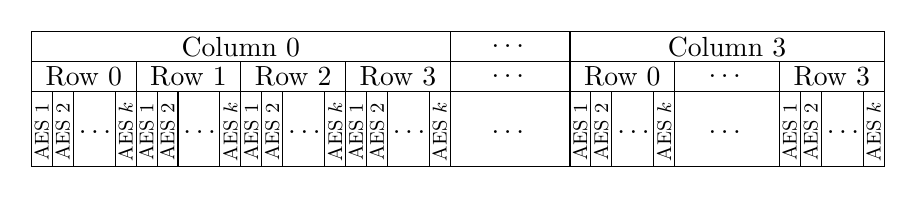
\begin{tikzpicture}[node distance=6em,auto,>=latex',scale=0.76]
  % Bottom
  
  \draw (0,0.75) rectangle (14.25,2);
  
  \draw (0,0.75) rectangle (0.35,2);
  \node[rotate=90,scale=0.8] at (0.175, 1.325) {\small AES 1};
  \draw (0.35,0.75) rectangle (0.7,2);
  \node[rotate=90,scale=0.8] at (0.525, 1.325) {\small AES 2};
  \node at (1.1, 1.325) {\ldots};
  \draw (1.4,0.75) rectangle (1.75,2);
  \node[rotate=90,scale=0.8] at (1.575, 1.325) {\small AES $k$};
  
  \draw (1.75,0.75) rectangle (2.1,2);
  \node[rotate=90,scale=0.8] at (1.925, 1.325) {\small AES 1};
  \draw (2.1,0.75) rectangle (2.45,2);
  \node[rotate=90,scale=0.8] at (2.275, 1.325) {\small AES 2};
  \node at (2.85, 1.325) {\ldots};
  \draw (3.15,0.75) rectangle (3.5,2);
  \node[rotate=90,scale=0.8] at (3.325, 1.325) {\small AES $k$};
  
  \draw (3.5,0.75) rectangle (3.85,2);
  \node[rotate=90,scale=0.8] at (3.675, 1.325) {\small AES 1};
  \draw (3.85,0.75) rectangle (4.2,2);
  \node[rotate=90,scale=0.8] at (4.025, 1.325) {\small AES 2};
  \node at (4.6, 1.325) {\ldots};
  \draw (4.9,0.75) rectangle (5.25,2);
  \node[rotate=90,scale=0.8] at (5.075, 1.325) {\small AES $k$};
  
  \draw (5.25,0.75) rectangle (5.6,2);
  \node[rotate=90,scale=0.8] at (5.425, 1.325) {\small AES 1};
  \draw (5.60,0.75) rectangle (5.95,2);
  \node[rotate=90,scale=0.8] at (5.775, 1.325) {\small AES 2};
  \node at (6.35, 1.325) {\ldots};
  \draw (6.65, 0.75) rectangle (7,2);
  \node[rotate=90,scale=0.8] at (6.825, 1.325) {\small AES $k$};
    
  \node at (8, 1.325) {\ldots};
  
  \draw (9,0.75) rectangle (9.35,2);
  \node[rotate=90,scale=0.8] at (9.175, 1.325) {\small AES 1};
  \draw (9.35,0.75) rectangle (9.7,2);
  \node[rotate=90,scale=0.8] at (9.525, 1.325) {\small AES 2};
  \node at (10.1, 1.325) {\ldots};
  \draw (10.4,0.75) rectangle (10.75,2);
  \node[rotate=90,scale=0.8] at (10.575, 1.325) {\small AES $k$};
  
  \node at (11.625, 1.325) {\ldots};
  
  \draw (12.5,0.75) rectangle (12.85,2);
  \node[rotate=90,scale=0.8] at (12.675, 1.325) {\small AES 1};
  \draw (12.85,0.75) rectangle (13.2,2);
  \node[rotate=90,scale=0.8] at (13.025, 1.325) {\small AES 2};
  \node at (13.6, 1.325) {\ldots};
  \draw (13.9,0.75) rectangle (14.25,2);
  \node[rotate=90,scale=0.8] at (14.075, 1.325) {\small AES $k$};
  
  % Middle
  \draw (0,2) rectangle (1.75,2.5);
  \node at (0.875, 2.25) {Row 0};
  \draw (1.75,2) rectangle (3.5,2.5);
  \node at (2.625, 2.25) {Row 1};
  \draw (3.5,2) rectangle (5.25,2.5);
  \node at (4.375, 2.25) {Row 2};
  \draw (5.25,2) rectangle (7,2.5);
  \node at (6.125, 2.25) {Row 3};
  \node at (8, 2.25) {\ldots};
  \draw (9,2) rectangle (10.75,2.5);
  \node at (9.875, 2.25) {Row 0};
  \draw (10.75,2) rectangle (12.5,2.5);
  \node at (11.625, 2.25) {\ldots};
  \draw (12.5,2) rectangle (14.25,2.5);
  \node at (13.375, 2.25) {Row 3};
  
  
  % Top
  \draw (0,2.5) rectangle (7,3);
  \node at (3.5, 2.75) {Column 0};
  \draw (7,2.5) rectangle (9,3);
  \node at (8, 2.75) {\ldots};
  \draw (9,2.5) rectangle (14.25,3);
  \node at (11.625, 2.75) {Column 3};
  \end{tikzpicture}
  \caption{Bit ordering in $\vec m_i$ in the \bwbs{} representation}
  \label{fig:bwbs-state}
\end{figure}

The $\AddRoundKey$ stage performs a XOR between the AES state and the
current round key. This operation only consists of $8$ $\Add$
operations.  
To minimize the
number of $\Recrypt$, we perform the $\Recrypt$ operation only on $9$ of
the temporary variables and on the $8$ outputs. In total, this stage
costs $83$ $\Add$, $32$ $\Mult$ and $17$
$\Recrypt$. In order to compute the \emph{minimal} number of $\Recrypt$ needed to homomorphically evaluate a given circuit, we refer you to~\cite{LP2013}.

The $\ShiftRows$ stage consists in performing a permutation of the
state. For this we add the $\sigma^\zeta_i$'s of the associated
permutation $\zeta$ in the public key, and the rotation is performed 
at no additional cost during the final $\Recrypt$ of the $\SubBytes$
stages. 
Finally the $\MixColumns$ stage requires $3$ permutations of the AES
state; it requires a total of $3\times 8=24$ $\Recrypt$
and $38$ $\Add$, and the addition of the $\sigma^\zeta_i$'s of
three permutations $\zeta$ to the public key. 

In total, our byte-wise implementation of AES requires  $1260$ $\Add$,
 $320$ $\Mult$, and $377$ $\Recrypt$.

\paragraph{State-Wise Bitslicing.} In this representation, each of the
$128$ bits of the AES state is stored in a different ciphertext. One
can then perform $k=\ell$ AES encryptions in parallel. This
corresponds to a full bitslice implementation of AES.
More precisely
the AES state is composed of $128$ ciphertexts $c_0,\ldots,c_{127}$,
where the underlying plaintexts $\vec m_0,\ldots,\vec m_{127}$ are
such that $\vec m_{i+j\cdot 8}[k]$ is the $i$-th bit of the $j$-th
byte of the state of the $k$-th AES.

The $\AddRoundKey$ stage requires $128$ $\Add$ operations. The
$\SubBytes$ stage is implemented using the same circuit as
above. Since the circuit needs to be evaluated on each of the $16$
bytes of the AES state,  the stage costs 
$16\times83=1328$ $\Add$, $16\times32 = 512$
$\Mult$, and $16\times17=272$ $\Recrypt$. The $\ShiftRows$ stage consists in
performing a permutation of the state, and this is done by permuting
the indices of bits in the homomorphic AES state at no additional
cost. The 
$\MixColumns$ stage 
requires  $608$ $\Add$. The total cost the AES evaluation is then $14688$
$\Add$,  $5120$
$\Mult$ and $2448$ $\Recrypt$. 

\begin{table}[tb]\centering
\caption{Timings of byte-wise and state-wise homomorphic AES developed in
  C++ with GMP,
  running on a desktop computer (Intel Core i7 at 3.4Ghz, 32GB RAM).}
\label{table:aes-results}
\subtable[Timings for byte-wise representation]{
\begin{tabular}{|l|c|c|c|c|c|c|c|c|c|}
\hline \textbf{Instance}&$\lambda$&$\ell$&$\#$ of enc.&
\textsf{Add-}&$\ShiftRows$&\textsf{Mix-}&\textbf{Total AES}&\textbf{Relative}\\
&&&in parallel&\textsf{RoundKey}&\& $\SubBytes$&\textsf{Columns}&(in hours)&\textbf{time}\\\hline
\hline
%\textbf{Toy}&$42$&$16$&$1$&$0.006$s&{$2.2$s}&$3$s&$\mathbf{0.013}$&48s\\\hline
\textbf{Small}&$52$&$48$&$3$&$0.04$s&{$21$s}&$29$s&$\mathbf{0.125}$&2min 30s\\\hline
\textbf{Medium}&$62$&$144$&$9$&$0.3$s&$210$s&$290$s&$\mathbf{1.25}$&8min 20s\\\hline
\textbf{Large}&$72$&$528$&$33$&$1.6$s&$2970$s&$4165$s&$\mathbf{18.3}$&33min\\\hline
\end{tabular}
}

\subtable[Timings for state-wise representation]{

\begin{tabular}{|l|c|c|c|c|c|c|c|c|c|}
\hline \textbf{Instance}&$\lambda$&$\ell$&$\#$ of enc.&\textsf{Add-}&\textsf{Sub-}&\textsf{Shift-}&\textsf{Mix-}&\textbf{Total AES}&\textbf{Relative}\\
&&&in parallel&\textsf{RoundKey}&\textsf{Bytes}&\textsf{Rows}&\textsf{Columns}&(in hours)&\textbf{time}\\\hline
\hline
%\textbf{Toy}&$42$&$10$&$10$&$0.06$s&$33$s&$0$s&$0.02$s&$\mathbf{0.08}$&$29$s\\\hline
\textbf{Small}&$52$&$37$&$37$&$0.06$s&$309$s&$0$s&$0.09$s&$\mathbf{0.74}$&1min 12s\\\hline
\textbf{Medium}&$62$&$138$&$138$&$4.5$s&$3299$s&$0$s&$0.44$s&$\mathbf{7.86}$&3min 25s\\\hline
\textbf{Large}&$72$&$531$&$531$&$27$s&$47656$s&$0.04$s&$2.8$s&$\mathbf{113}$&{12min 46s}\\\hline

\end{tabular}
}
\end{table}

\paragraph{Implementation Results.} We implemented both variants
using the concrete parameters from Table~\ref{t:concparams}; our
results are summarized in 
Table~\ref{table:aes-results}. The 
relative time is the total time of AES evaluation divided  by the
number of encryptions processed in parallel. Notice that the \swbs variant
yields  better relative times. 

Our timings are comparable to~\cite{GHS2012c} for the RLWE-based scheme, where a relative time of $5$ minutes per block is
reported; the authors used a $24$-core server with 256GB of RAM, while
our program runs on a more modest desktop computer with 4 cores and
32GB of RAM (the whole public key fits in RAM).
We claim a slightly lower security level, however: $72$ bits versus $80$
bits for the implementation from~\cite{GHS2012c}.

%
\bibliographystyle{plain}
\bibliography{batchdghv}

\end{document}

